%=========================================================
% Peripheral : GPIO
%=========================================================
\section{Peripheral : GPIO}

\begin{description}

    \item[Overview]\mbox{}\\
        GPIO (module name PORT) has 3 x 32bit input / output ports. Each pin direction can be configured respectively.             

    \item[Input / Output Signals]\mbox{}\\
        Input / Output signals of GPIO (PORT) are shown in Table \ref{tb:IOSIGNALS_GPIO}. The I/O buffers for each GPIOn signal are implemented in the GPIO module.
        
%-------------------------------
\begin{table}[H]
    \begin{adjustbox}{scale={0.65}{0.8}}
    \textsf{
    \begin{tabular}{|L{4cm}{2cm}{t}|L{4cm}{2cm}{t}|L{2cm}{1cm}{t}|L{7cm}{6cm}{t}|L{10cm}{6cm}{t}|L{3cm}{2cm}{t}|}
        \hline
        %-------------------------------------
        \rowcolor{LightPurple}
        \textbf{Group} &
        \textbf{Direction} &
        \textbf{Width} &
        \textbf{Name} &
        \textbf{Description} &
        \textbf{Note}
        \nextRow \hline
        %-------------------------------------
        System & input  & ~ & RES & Reset & ~
        \nextRow \hline
        %-------------------------------------
        System & input  & ~ & CLK & System Clock & ~
        \nextRow \hline
        %-------------------------------------
        AHB    & input  & ~                   & S\_HSEL      & AHB Lite Slave Select & ignored
        \nextRow \hline
        %-------------------------------------
        AHB    & input  & \lbrack  1:0\rbrack & S\_HTRANS    & AHB Lite Slave Transfer Type & ~
        \nextRow \hline
        %-------------------------------------
        AHB    & input  & ~                   & S\_HWRITE    & AHB Lite Slave Write & ~
        \nextRow \hline
        %-------------------------------------
        AHB    & input  &                     & S\_HMASTLOCK & AHB Lite Slave Locked Transfer & ignored
        \nextRow \hline
        %-------------------------------------
        AHB    & input  & \lbrack  2:0\rbrack & S\_HSIZE     & AHB Lite Slave Access Size & ~
        \nextRow \hline
        %-------------------------------------
        AHB    & input  & \lbrack  2:0\rbrack & S\_HBURST    & AHB Lite Slave Burst Access & ignored
        \nextRow \hline
        %-------------------------------------
        AHB    & input  & \lbrack  3:0\rbrack & S\_HPROT     & AHB Lite Slave Protection & ignored
        \nextRow \hline
        %-------------------------------------
        AHB    & input  & \lbrack 31:0\rbrack & S\_HADDR     & AHB Lite Slave Address & ~
        \nextRow \hline
        %-------------------------------------
        AHB    & input  & \lbrack 31:0\rbrack & S\_HWDATA    & AHB Lite Slave Write Data & ~
        \nextRow \hline
        %-------------------------------------
        AHB    & input  & ~                   & S\_HREADY    & AHB Lite Slave Ready Input & ~
        \nextRow \hline
        %-------------------------------------
        AHB    & output & ~                   & S\_HREADYOUT & AHB Lite Slave Ready Output & ~
        \nextRow \hline
        %-------------------------------------
        AHB    & output & \lbrack 31:0\rbrack & S\_HRDATA    & AHB Lite Slave Read Data & ~
        \nextRow \hline
        %-------------------------------------
        AHB    & output & ~                   & S\_HRESP     & AHB Lite Slave Response & always output 0
        \nextRow \hline
        %-------------------------------------
        GPIO   & inout  & \lbrack 31:0\rbrack & GPIO0        & 32bit GPIO0 & ~
        \nextRow \hline
        %-------------------------------------
        GPIO   & inout  & \lbrack 31:0\rbrack & GPIO1        & 32bit GPIO1 & ~
        \nextRow \hline
        %-------------------------------------
        GPIO   & inout  & \lbrack 31:0\rbrack & GPIO2        & 32bit GPIO2 & ~
        \nextRow \hline
        %-------------------------------------
    \end{tabular}
    }
    \end{adjustbox}
    \caption{Input / Output Signals of GPIO(PORT)}
    \label{tb:IOSIGNALS_GPIO}
\end{table}
%-------------------------------

    \item[Control Registers]\mbox{}\\
        Controls registers of GPIO (PORT) are shown in Table \ref{tb:REG_GPIO_PDR0} to Table \ref{tb:REG_GPIO_PDD2}. The PDDn configures the direction of each pin; 0 for input, 1 for output. When a port bit is configured as an input, the read value of the data register PDRn corresponds to the input signal level. When a port bit is configured as an output, the read value of the data register PDRn is the register value, and the write value is stored in the data register PDRn and it is output to the corresponding external pin.

\end{description}

%-------------------------------
\begin{table}[H]
    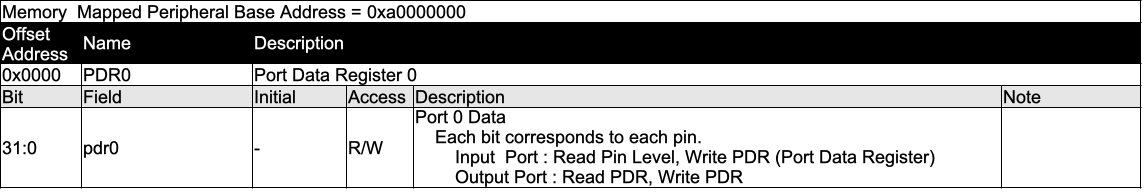
\includegraphics[width=1.0\columnwidth]{./Table/REG_GPIO_PDR0.png}
    \caption{PDR0}
    \label{tb:REG_GPIO_PDR0}
\end{table}
%-------------------------------
%-------------------------------
\begin{table}[H]
    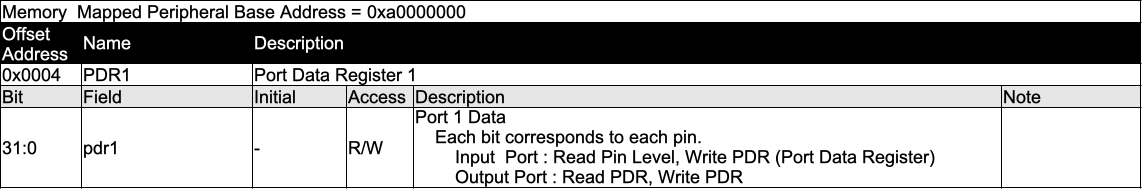
\includegraphics[width=1.0\columnwidth]{./Table/REG_GPIO_PDR1.png}
    \caption{PDR1}
    \label{tb:REG_GPIO_PDR1}
\end{table}
%-------------------------------
%-------------------------------
\begin{table}[H]
    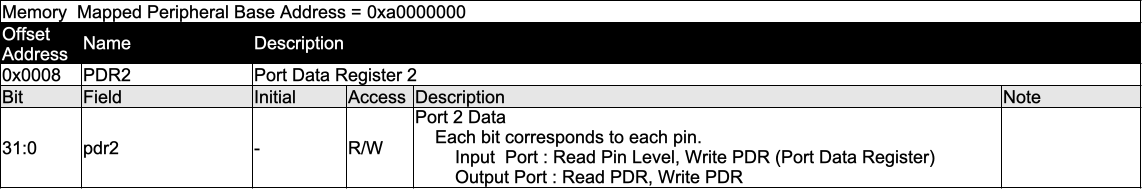
\includegraphics[width=1.0\columnwidth]{./Table/REG_GPIO_PDR2.png}
    \caption{PDR2}
    \label{tb:REG_GPIO_PDR2}
\end{table}
%-------------------------------
%-------------------------------
\begin{table}[H]
    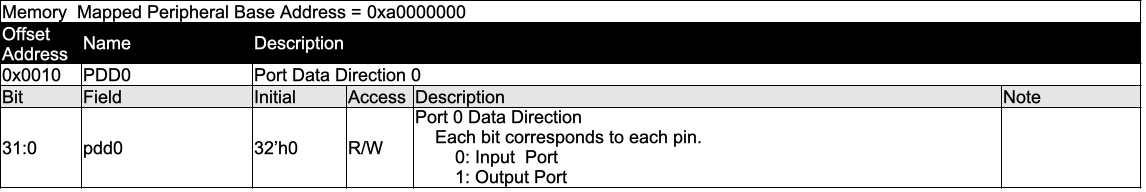
\includegraphics[width=1.0\columnwidth]{./Table/REG_GPIO_PDD0.png}
    \caption{PDD0}
    \label{tb:REG_GPIO_PDD0}
\end{table}
%-------------------------------
%-------------------------------
\begin{table}[H]
    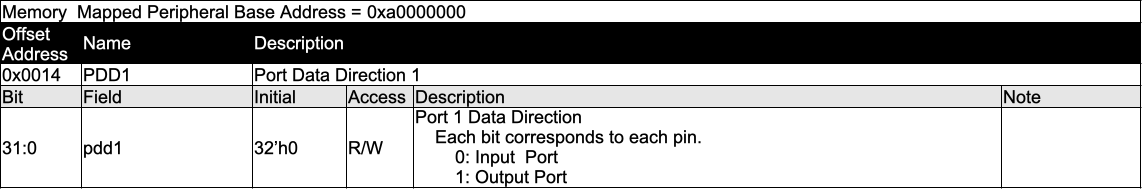
\includegraphics[width=1.0\columnwidth]{./Table/REG_GPIO_PDD1.png}
    \caption{PDD1}
    \label{tb:REG_GPIO_PDD1}
\end{table}
%-------------------------------
%-------------------------------
\begin{table}[H]
    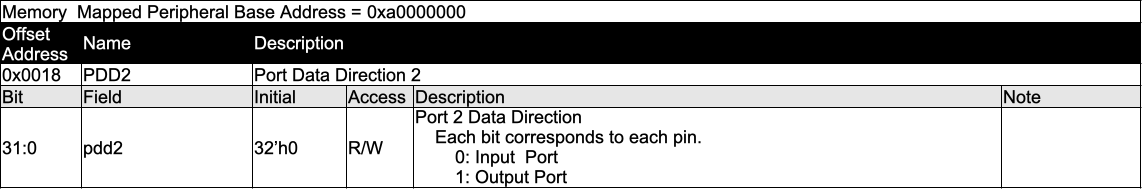
\includegraphics[width=1.0\columnwidth]{./Table/REG_GPIO_PDD2.png}
    \caption{PDD2}
    \label{tb:REG_GPIO_PDD2}
\end{table}
%-------------------------------

